% !TeX spellcheck = ru_RU
% !TEX root = vkr.tex

\section{Тестирование и оценка производительности}
\label{sec:testing-performance}

В данном разделе собраны методы проверки разработанной виртуальной машины и
оценка её производительности. 
\subsection{Методика тестирования}
\label{subsec:testing-methodology}


Тестирование виртуальной машины строилось как комбинация нескольких подходов,
которые проверяют разные классы свойств. Регрессионные тесты фиксируют уже
известные сценарии работы компилятора, стандартной библиотеки и среды
выполнения. Такие
тесты удобны для проверки повторяемости исправлений, но сами по себе покрывают
только заранее выбранные случаи.
% \begin{figure}[H]
%     \centering
%     \resizebox{\textwidth}{!}{\begin{tikzpicture}[
    node distance=14mm and 10mm,
    stage/.style={
        draw,
        rounded corners=2pt,
        semithick,
        align=center,
        minimum height=11mm,
        text width=20mm,
        fill=gray!8
    },
    snippetstage/.style={
        draw,
        line width=0.35pt,
        draw=black!30,
        minimum width=37mm,
        minimum height=24mm,
        fill=white
    },
    smstage/.style={
        draw,
        line width=0.35pt,
        draw=black!30,
        minimum width=37mm,
        minimum height=24mm,
        fill=white
    },
    vmstage/.style={
        draw,
        rounded corners=2pt,
        semithick,
        align=center,
        minimum height=30mm,
        text width=56mm,
        fill=gray!8
    },
    innerbox/.style={
        draw,
        align=center,
        fill=white,
        inner sep=3pt,
        text width=46mm
    },
    cell/.style={
        draw,
        minimum height=6mm,
        minimum width=12mm,
        align=center,
        fill=white,
        font=\ttfamily\scriptsize
    },
    tool/.style={
        draw,
        rounded corners=2pt,
        align=center,
        minimum height=8mm,
        text width=36mm,
        fill=white
    },
    flow/.style={->, semithick},
    attach/.style={->, dashed, semithick}
]

\node[snippetstage] (lama) {};
\node[stage, right=of lama, text width = 30mm] (compiler) {Компилятор\\байткода};
\node[smstage, right=of compiler] (bc) {};
\node[vmstage, right=of bc] (vm) {Виртуальная машина};
\node[anchor=north west, inner sep=0pt] at ($(lama.north west)+(0.8mm,-0.8mm)$) {
    \begin{tikzpicture}[x=1mm,y=-1mm]
        \clip (0,0) rectangle (36.4,21.9);
        \node[
            anchor=north west,
            align=left,
            font=\ttfamily\fontsize{4.6}{5.1}\selectfont
        ] at (0.05,0.05)
            {var x, y, z;\\
             \\
             fun zip (x) \{\\
             \ \ case x of Pair (x, y) ->\\
             \ \ \ \ case x of\\
             \ \ \ \ \ \ Nil          ->  Nil\\
             \ \ \ \ | Cons (x, xs) -> case y of\\
             \ \ \ \ \ \ \ \ \ \ \ \ \ \ \ Nil ->  Nil\\
             \ \ \ \ \ \ \ \ \ \ \ \ \ \ | Cons (y, ys) ->\\
             \ \ \ \ \ \ \ \ \ \ \ \ \ \ \ \ Cons (Pair (x, y),\\
             \ \ \ \ \ \ \ \ \ \ \ \ \ \ \ \ \ \ zip (Pair (xs, ys)))\\
             \ \ \ \ \ \ \ \ \ \ \ \ \ \ esac\\
             \ \ \ \ esac};
        \node[anchor=south east, font=\ttfamily\tiny, text=gray!65]
            at (36.8,21.5) {$\ddots$};
    \end{tikzpicture}
};
\node[anchor=north west, inner sep=0pt] at ($(bc.north west)+(0.8mm,-0.8mm)$) {
    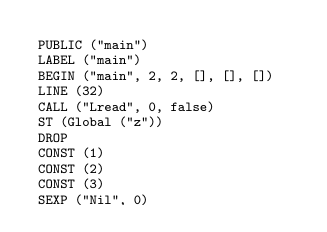
\begin{tikzpicture}[x=1mm,y=-1mm]
        \clip (0,0) rectangle (34.4,22.4);
        \node[
            anchor=north west,
            align=left,
            font=\ttfamily\fontsize{5.0}{5.6}\selectfont
        ] at (0.1,0.25)
            {PUBLIC ("main")\\
             LABEL ("main")\\
             BEGIN ("main", 2, 2, [], [], [])\\
             LINE (32)\\
             CALL ("Lread", 0, false)\\
             ST (Global ("z"))\\
             DROP\\
             CONST (1)\\
             CONST (2)\\
             CONST (3)\\
             SEXP ("Nil", 0)\\
             SEXP ("Cons", 2)};
    \end{tikzpicture}
};
\node[] at ([yshift=-11mm]vm.center) 
(ops)
{
    \begin{tikzpicture}[node distance=0mm]
        \node[cell] (c1) {insn$_1$};
        \node[cell, right=0mm of c1] (c2) {insn$_2$};
        \node[cell, right=0mm of c2, minimum width=8mm] (c3) {$\cdots$};
        \node[cell, right=0mm of c3] (c4) {insn$_n$};
    \end{tikzpicture}
};

\draw[flow] (lama) -- (compiler);
\draw[flow] (compiler) -- (bc);
\draw[flow] (bc) -- (vm);

\node[tool, below=16mm of lama, fill=green!12] (tool-lama) {\textsc{AFL++} \\Grammarinator};
\node[tool, below=16mm of bc, fill=orange!14] (tool-bc) {\textsc{AFL++}};
\node[tool, below=16mm of vm, fill=blue!10] (tool-cbmc) {\textsc{CBMC}};

\draw[attach] (tool-lama) -- (lama);
\draw[attach] (tool-bc) -- (bc);
\draw[attach] (tool-cbmc) -- (ops);

\node[font=\small, align=center, below=1mm of tool-lama] {фаззинг\\грамматики};
\node[font=\small, align=center, below=1mm of tool-bc] { фаззинг\\байткода};
\node[font=\small, align=center, below=1mm of tool-cbmc] {проверка инвариантов };

\end{tikzpicture}
}
%     \caption{Схема основных представлений программы и соответствующих методов анализа.}
%     \label{fig:fuzz-pipeline}
% \end{figure}

Для проверки корректности использовались два вида фаззинга. Первый подавал виртуальной машине
повреждённый байткод и проверял, что ошибки в заголовках, операндах и ссылках не приводят к авариям,
ошибкам памяти или неопределённому поведению. Второй порождал грамматически корректные программы Lama,
компилировал их в байткод и в нативную программу и сравнивал результаты исполнения. Такая схема
позволяла одновременно проверять устойчивость реализации к некорректным входам и согласованность её
семантики с существующей реализацией языка. В таблице \ref{tab:fuzz-comparison} приведены результаты данных
методов тестирования.
\begin{table}[H]
    \def\arraystretch{1.1}
    \centering
    \caption{Сравнение результатов байткодного и грамматического фаззинга}
    \label{tab:fuzz-comparison}
    \resizebox{\textwidth}{!}{%
    \begin{tabular}{lcc}
        \toprule
        Метрика & Байткодный фаззинг & Грамматический фаззинг \\
        \midrule
        Длительность кампании, ч & \num{17.6} & \num{20.6} \\
        Суммарная скорость, исп/с & \num{1854.5} & \num{61.7} \\
        Общее число запусков & \num{117803305} & \num{4564820} \\
        Покрытие строк, \% & \num{68.5} & \num{75.4} \\
        Исправления & 8 & 1 \\
        \bottomrule
    \end{tabular}
    }
\end{table}
 

Более подробно методика тестирования описана в предыдущей работе~\cite{ParfenovPractice2026}. 
\subsection{Оценка производительности}

Целью данного раздела является оценка производительности реализованной виртуальной машины. В рамках эксперимента были поставлены следующие вопросы:
\begin{description}
  \item[RQ1:] Каковы временные накладные расходы виртуальной машины относительно нативного исполнения?
  \item[RQ2:] Каковы накладные расходы виртуальной машины по памяти относительно нативного исполнения?
\end{description}

\subsubsection{Набор данных и оборудование}
Для проведения экспериментов были использованы пять программ на Lama разного объема и сложности:
\begin{itemize}
  \item \textbf{Sort.lama} --- сортировка пузырьком массива чисел
  \item \textbf{Ackermann.lama} --- вычисление значений функции Аккермана
  \item \textbf{GenCyclicArray.lama} --- построение и сравнение циклических массивов
  \item \textbf{Компилятор Lama на Lama} --- в качестве входных данных будут использоваться его тесты:
    \begin{itemize}
      \item \textbf{regression/} --- основной набор регрессионных тестов компилятора Lama на корректность исполнения программ. 
      \item \textbf{regression/expressions} --- автоматически сгенерированные программы, состоящие в основном из простых выражений.
    \item \textbf{regression/deep-expressions} --- автоматически сгенерированные программы с глубоко вложенными выражениями.

    \end{itemize}
\end{itemize}

Эксперименты проводились на следующем тестовом оборудовании:
  \begin{itemize}
    \item ЦПУ: AMD Ryzen 7 6800H
    \begin{itemize}
      \item каждый запуск привязывался к одному физическому ядру (без одновременной многопоточности)
    \end{itemize}
    \item ОЗУ: DDR5 16 ГБ @ 6400 МГц
    \begin{itemize}
      \item без подкачки
    \end{itemize}
    \item ОС: Ubuntu 26.04 x86\_64
    \item Компилятор gcc версии Ubuntu 15.2.0-16ubuntu1
  \end{itemize}

Все измерения повторялись 20 раз. Для времени исполнения и пикового
  потребления памяти в качестве основной оценки использовалась медиана по
  запускам. Для времени дополнительно приводятся первый и третий квартили.

\label{subsec:performance-methodology}

\subsubsection{Эксперимент}




\subsection{Анализ выявленных ошибок и ограничений}
\label{subsec:testing-limitations}

